\section{Related Work}
\label{sec:related_work}

\begin{figure*}[h]
    \centering
    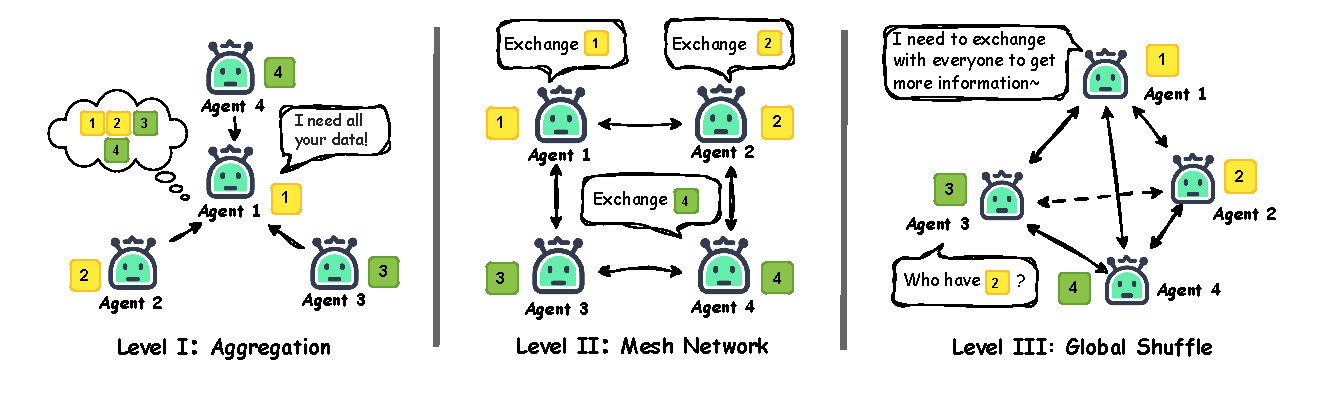
\includegraphics[width=1.0\textwidth]{figures/benchmark.pdf}
    \caption{Three complexity levels in \silobench{} characterized by their communication patterns. \textbf{Level I (Aggregation)}: A central agent collects data from all peers via a star topology. \textbf{Level II (Mesh Network)}: Agents exchange information with immediate neighbors through pairwise communication. \textbf{Level III (Global Shuffle)}: All agents must communicate with every other agent, requiring full mesh connectivity.}
    \label{fig:task_levels}
\end{figure*}


\paragraph{Context Limitations and Distributed Reasoning.}
The finite context window of LLMs constitutes a fundamental bottleneck for processing large-scale information. While recent advances have extended context lengths to millions of tokens \citep{reid2024gemini,liuworld}, the quadratic computational complexity of attention mechanisms makes centralized processing increasingly resource-intensive and prone to ``lost-in-the-middle'' phenomena \citep{liu2024lost}. 
Although Retrieval-Augmented Generation (RAG) offers a palliative solution \citep{wang2024m,islam2024open}, it often fractures global context, struggling with tasks that require holistic reasoning across disjoint segments. 
Existing benchmarks like SCROLLS \citep{shaham2022scrolls}, LongBench \citep{bai2024longbench}, and \(\infty\)Bench \citep{zhang2024infty} effectively evaluate single-agent retrieval but overlook the paradigm of \textit{distributed collaboration}. 
We posit that overcoming the context barrier requires shifting from centralized attention to collaborative computation, where agents act as distributed processors, to digest partitioned information and synthesize global insights, which is a capability currently unmeasured by standard long-context evaluations.

\paragraph{Multi-Agent Architectures and Role-Agnosticism.}
The paradigm of orchestrating multiple LLM agents has evolved from simple role-playing to complex problem-solving frameworks. 
Foundational works like CAMEL \citep{li2023camel} and MetaGPT \citep{hong2023metagpt} utilize \textit{role-specialized agents} (e.g., assigning ``Manager'' or ``Coder'' personas) embedded within fixed hierarchical or waterfall workflows. 
While effective for domain-specific tasks like software engineering \citep{islam2024mapcoder} and interactive image generation \citep{ma2025talk2image}, these approaches entangle the agents' reasoning capabilities with semantic role priors, making it difficult to isolate the contribution of the communication architecture itself. 
Other efforts, such as debate-based systems \citep{du2023improving} or Mixture-of-Agents \citep{wangmixture,su2026daao}, often prescribe static topological constraints that limit dynamic information flow. 
\textbf{We introduce \silobench{}, a role-agnostic configurable environment with task-structural guidance for evaluating distributed coordination under information silos.} 
Unlike static test suites that prescribe fixed roles and communication scripts, our framework dynamically generates unlimited evaluation instances while providing high-level task hints, allowing observation of whether agents can translate structural understanding into effective coordination protocols \cite{presstrain,liuagentbench}.



